\documentclass[12 pt]{article}        	
\usepackage{amsfonts, amssymb, amsmath, graphicx, pgfplots, tikz}
\pgfplotsset{compat=1.17}

\oddsidemargin=-0.5cm

\setlength{\textwidth}{6.5in}         	
\addtolength{\voffset}{-20pt}        	
\addtolength{\headsep}{25pt}

\pagestyle{myheadings}

\markright{Juan Ignacio Elosegui \hfill Práctica 6 \hfill}

\begin{document}

\section*{Ejercicio 1}
    \begin{center}
        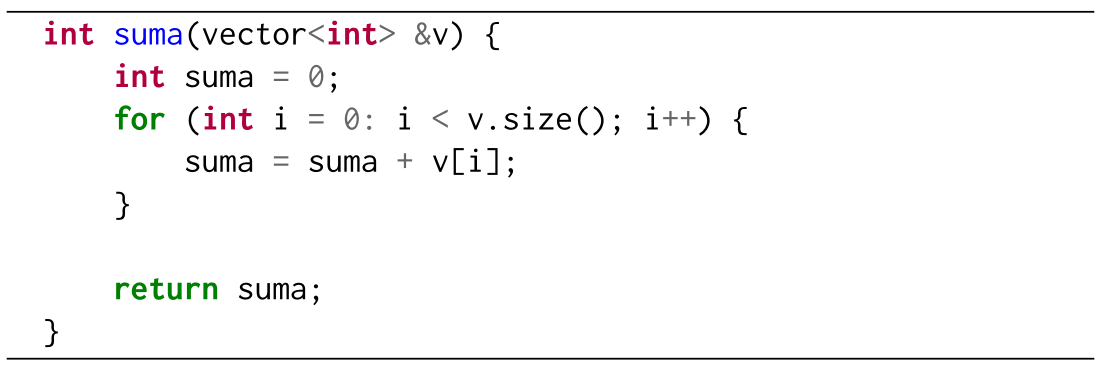
\includegraphics[width=0.7 \linewidth]{img/ej1.png}
    \end{center}
    \begin{itemize}
        \item \textbf{Definir el tamaño de entrada $n$.} \\
        El tamaño de entrada $n$ es el tamaño del vector $v$.
        \item \textbf{Identificar el peor caso de ejecución del programa.} \\
        Todos los casos son los peores, entre más grande sea $|v|$, más tardará en ejecutar el programa.
        \item \textbf{Escribir la función de costo temporal $\mathcal{T}(n)$ asociada al peor caso.} \\
        \(\mathcal{T}(n) = (1) + (1) + n(4 + 3 + 6) + (1)\) \\
        \(\implies \mathcal{T}(n) = 3 + n(13)\) \\
        \(\therefore \mathcal{T}(n) = 13n+3\) \\
        Las declaraciones tienen un costo de 1, que es el primer paréntesis. \\
        En el segundo paréntesis también, es el \texttt{int i = 0} que se hace una sola vez en el ciclo \texttt{for}. \\
        Luego, se hace la comparación, acceso a \texttt{i}, acceso a \texttt{v} y la operación \texttt{.size()}. Esto tiene un costo de 4 que se ejecuta $n$ veces. También se ejecuta $n$ veces cuando se actualiza la variable \texttt{suma}: el acceso a la variable \texttt{suma} y \texttt{v}, sumado al operador + e =, y el acceso a la posición \texttt{i} hace que tenga un costo esta línea de 6. Luego se incrementa \texttt{i}, se accede, se suma uno y se vuelve a guardar con un costo de \texttt{3}. \\
        Finalmente, se devuelve la variable \texttt{suma}, que en los \texttt{return} tiene un costo de 1.
        \item \textbf{Proponer un orden de complejidad $\mathcal{O}$ para $\mathcal{T}(n)$.} \\
        \(\mathcal{T}(n) = 13n+3 \in O(n)\)
        \item \textbf{Mostrar que $\mathcal{T}(n)$ pertenece al órden de complejidad propuesto.} \\
        Quiero verificar que: \\
        \(0 \leq \mathcal{T}(n) \leq c \cdot O(n), (\forall n \geq n_{0})\) \\
        \(\implies 0 \leq 13n+3 \leq c \cdot n\) \\
        Sabemos que $13n+3$ es estrictamente creciente, por lo tanto, será siempre mayor o igual a cero con un $n_{0} \geq 0$. \\
        \(\implies 13n+3 \leq c \cdot n\) \\
        \(\implies \frac{13n+3}{n} \leq c\) \\
        Ya cuando despejo, puedo usar el $n_{0}$. \\
        \(\implies 13+\frac{3}{n_{0}} \leq c\) \\
        Si tomamos que \(n_{0} = 1 \wedge c = 16\), vemos que se cumple para todo $n \geq n_{0}$.
        \begin{center}
            \begin{tikzpicture}
                \begin{axis}[
                    domain=0:10,   % Rango del eje x
                    samples=,  % Número de muestras para suavidad
                    axis lines=middle, % Dibujar los ejes en el centro
                    xlabel={$n$}, % Etiqueta del eje x
                    legend style={at={(1.05,1)}, anchor=north west}, % Posición de la leyenda
                    width=10cm, height=7cm, % Tamaño del gráfico
                    ]
                    % Graficar la función T(n)
                    \addplot[blue, thick] {13*x+3};
                    \addlegendentry{$\mathcal{T}(n) = 13n + 3$}
                
                    % Graficar la función O(n)
                    \addplot[red, thick, dashed] {16*x};
                    \addlegendentry{$O(n) = 16n$}
                \end{axis}
            \end{tikzpicture}                
            \(\therefore \mathcal{T}(n) = 13n+3 \in O(n)\)
        \end{center}
    \end{itemize}

\newpage

\section*{Ejercicio 2}
    \begin{center}
        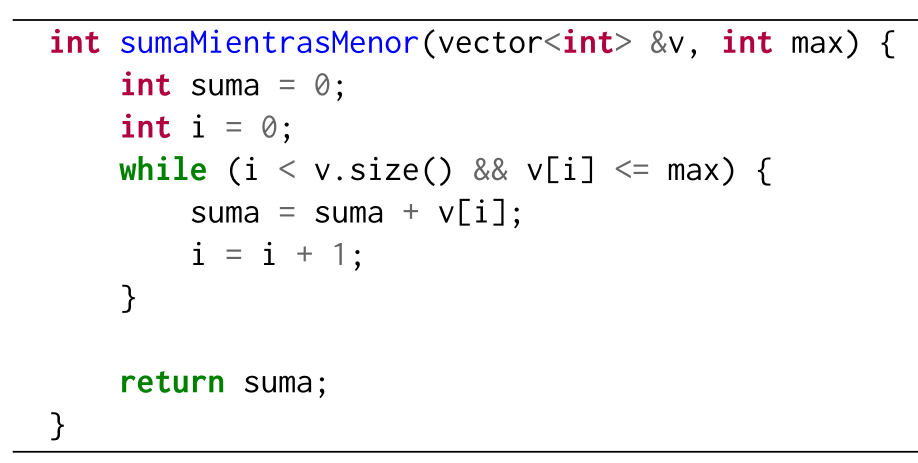
\includegraphics[width=0.7 \linewidth]{img/ej2.png}
    \end{center}
    \begin{itemize}
        \item \textbf{Definir el tamaño de entrada $n$.} \\
            El tamaño de entrada $n$ será el tamaño del vector \texttt{v}, llamado $|v|$.
        \item \textbf{Identificar el peor caso de ejecución del programa.} \\
            El peor caso es si \texttt{max} es mayor a todos los elementos del vector \texttt{v}. En este caso, el ciclo iterará más veces porque todos los elementos serán menores a \texttt{max}.
        \item \textbf{Escribir la función de costo temporal $\mathcal{T}(n)$ asociada al peor caso.} \\
            La definición de las variables en la primera y segunda línea tienen un costo de 1 cada una. \\
            En la comparación \texttt{i < v.size()} se debe acceder a las dos variables, acceder al valor de una y después compararlas, por lo que tiene un costo de 4. En la comparación \texttt{v[i] <= max} se accede a tres variables, se accede a un valor guardado en una, y se comparan, por lo que tiene un valor de 5. \\
            Dentro del \texttt{while}, se accede en la primera línea a cuatro variables, se suman y se guarda en una variable. Esto tiene un costo de 6. \\
            Se incrementa \texttt{i}, se accede a ella, se le suma uno y se guarda. Tiene un costo esto de 3. Esto se ejecuta $n$ veces. \\
            Finalmente, se devuelve \texttt{suma} con costo 1. \\
            \\
            \(\mathcal{T}(n) = (1+1)+(4+5+6+3)\cdot n+(4+5)+(1)\) \\
            Incluyo la negación de la guarda (es el $4+5$ después de la multiplicación) \\
            \(\implies \mathcal{T}(n) = (2)+(18)\cdot n+(9)+(1)\) \\
            \(\implies \mathcal{T}(n) = (2)+(18)\cdot n+10\) \\
            \(\therefore \mathcal{T}(n) = 18n+12\)
        \item \textbf{Proponer un orden de complejidad $\mathcal{O}$ para $\mathcal{T}(n)$.} \\
            \(\mathcal{T}(n) \in O(n)\)
        \item \textbf{Mostrar que $\mathcal{T}(n)$ pertenece al orden de complejidad propuesto.} \\
            Quiero probar que \(0 \leq \mathcal{T}(n) \leq c \cdot O(n), (\forall n \geq n_{0})\). \\
            \(\implies 0 \leq 18n+12 \leq c \cdot n, (\forall n \geq n_{0})\) \\
            \(\implies 0 \leq 18n+12\) Vale porque $18n+12$ es estrictamente creciente. \\
            \(\implies 18n+12 \leq c \cdot n, (\forall n \geq n_{0})\) \\
            \(\implies \frac{18n+12}{n} \leq c, (\forall n \geq n_{0})\) \\
            \(\implies 18+\frac{12}{n_{0}} \leq c, (\forall n \geq n_{0})\) \\
            Si tomo \(n_{0} = 1 \wedge c = 30\), se cumple la desigualdad para todo $n \geq n_{0}$.
            \begin{center}
                \begin{tikzpicture}
                    \begin{axis}[
                        domain=0:4,   % Rango del eje x
                        samples=,  % Número de muestras para suavidad
                        axis lines=middle, % Dibujar los ejes en el centro
                        xlabel={$n$}, % Etiqueta del eje x
                        legend style={at={(1.05,1)}, anchor=north west}, % Posición de la leyenda
                        width=10cm, height=7cm, % Tamaño del gráfico
                        ]
                        % Graficar la función T(n)
                        \addplot[blue, thick] {18*x+12};
                        \addlegendentry{$\mathcal{T}(n) = 18n + 12$}
                    
                        % Graficar la función O(n)
                        \addplot[red, thick, dashed] {30*x};
                        \addlegendentry{$O(n) = 30n$}
                    \end{axis}
                \end{tikzpicture}                
                \(\therefore \mathcal{T}(n) = 18n+12 \in O(n)\)
            \end{center}
    \end{itemize}

\newpage

\section*{Ejercicio 3}
    \begin{center}
        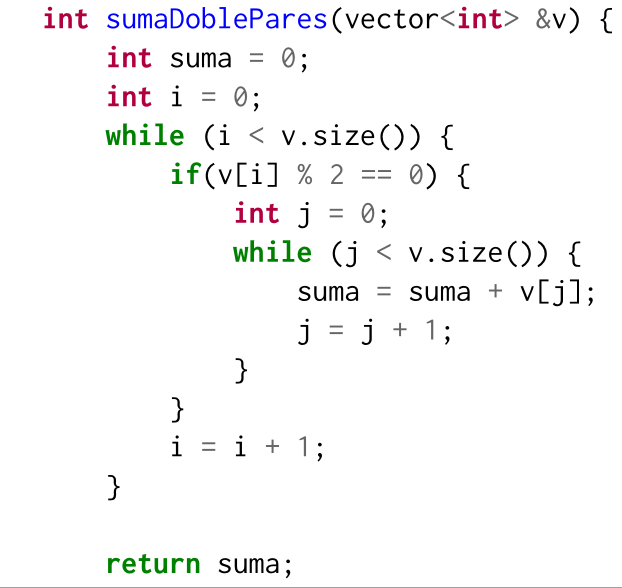
\includegraphics[width=0.7 \linewidth]{img/ej3.png}
    \end{center}
    \begin{itemize}
        \item \textbf{Definir el tamaño de entrada $n$.} \\
            El tamaño de la entrada es \texttt{|v|}.
        \item \textbf{Identificar el peor caso de ejecución del programa.} \\
            El peor caso sucede si tiene todos elementos pares el vector. En ese caso, si se encuentra un par, suma todos los elementos a la variable \texttt{suma} hasta el final del vector. Entre más pares haya, más operaciones hará.
        \item \textbf{Escribir la función de costo temporal $\mathcal{T}(n)$ asociada al peor caso.} \\
            Definición de las variables \texttt{suma} e \texttt{i} tienen un costo de 1. \\
            En la guarda del primer while, se accede a dos variables, se hace una operación en una y se hace una comparación. Esto tiene un costo de 4. \\
                En el \texttt{if} se accede a dos variables, se hace una operación y se hace una comparación. Esto tiene un costo de 4. \\
                    Se define una variable con costo 1. \\
                    En la guarda del segundo while, se accede a dos variables, se hace una operación en una y se hace una comparación. Esto tiene un costo de 4. \\
                        Se acceden a tres variables, se hace una operación, y se guarda el valor. Esto tiene un costo de 5. \\
                        Se accede a \texttt{j} y se hace una operación. Tiene un costo de 2. \\
                    Se incrementa la variable \texttt{i} en uno. Costo de 2. \\
                    Finalmente, se devuelve la variable \texttt{suma} con costo 1. \\
            \\
            \(\mathcal{T}(n) = (1+1)+(4+4+1+4+2+1+(5+2)\cdot n)\cdot n+(4)+(1)\) \\
            \(\implies \mathcal{T}(n) = (16+7n)\cdot n+7\) \\
            \(\therefore \mathcal{T}(n) = 16n+7n^{2}+7\)
        \item \textbf{Proponer un orden de complejidad $\mathcal{O}$ para $\mathcal{T}(n)$.} \\
            \(\mathcal{T}(n) \in O(n^{2})\)
        \item \textbf{Mostrar que $\mathcal{T}(n)$ pertenece al orden de complejidad propuesto.} \\
            Quiero probar que \(0 \leq \mathcal{T}(n) \leq c \cdot O(n^{2}), (\forall n \geq n_{0})\) \\
            \(\implies 0 \leq 16n+7n^{2}+7 \leq c \cdot n^{2}, (\forall n \geq n_{0})\) \\
            \(\implies 0 \leq 16n+7n^{2}+7 (\forall n \geq n_{0})\) Vale, porque $16n+7n^{2}+7$ es una función creciente.\\
            \(\implies 7n^{2}+16n+7 \leq c \cdot n^{2}, (\forall n \geq n_{0})\) \\
            \(\implies \frac{7n^{2}+16n+7}{n^{2}} \leq c, (\forall n \geq n_{0})\) \\
            \(\implies 7+\frac{16}{n_{0}}+\frac{7}{n^{2}_{0}} \leq c, (\forall n \geq n_{0})\) \\
            Si tomamos que \(n_{0} = 1 \wedge c = 30\), se cumple la desigualdad para todo $n \geq n_{0}$.
            \begin{center}
                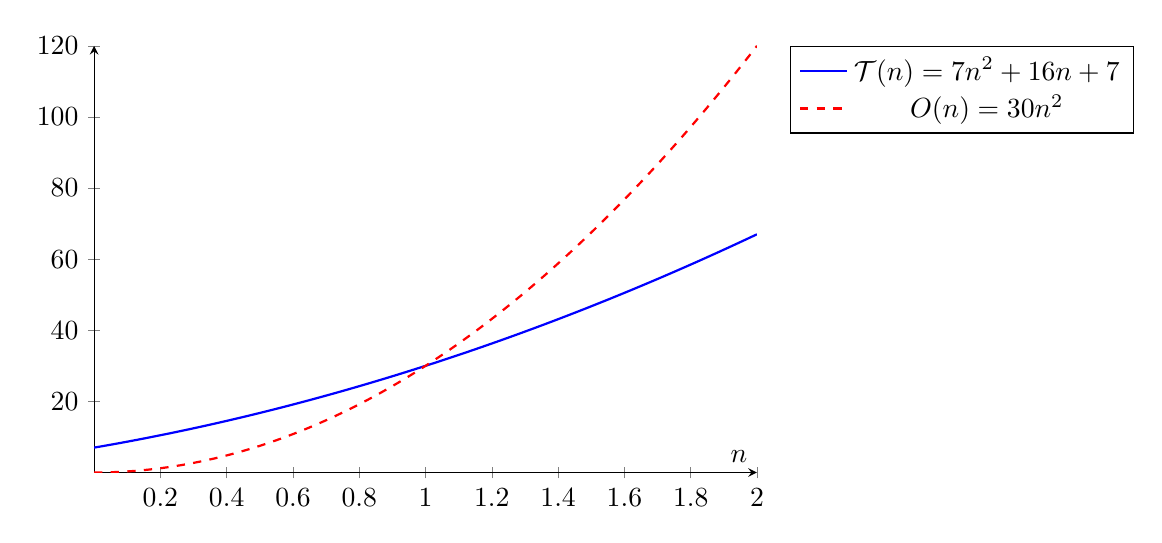
\begin{tikzpicture}
                    \begin{axis}[
                        domain=0:2,           % Rango del eje x
                        samples=100,            % Número de muestras para suavidad
                        axis lines=middle,      % Dibujar los ejes en el centro
                        xlabel={$n$},           % Etiqueta del eje x
                        ylabel={},              % Etiqueta del eje y
                        legend style={at={(1.05,1)}, anchor=north west}, % Posición de la leyenda
                        width=10cm, height=7cm, % Tamaño del gráfico
                        ]
                        % Graficar la función T(n)
                        \addplot[blue, thick] {7*x^2 + 16*x + 7};
                        \addlegendentry{$\mathcal{T}(n) = 7n^{2}+16n+7$}
                        
                        % Graficar la función O(n)
                        \addplot[red, thick, dashed] {30*x^2};
                        \addlegendentry{$O(n) = 30n^2$}
                    \end{axis}
                \end{tikzpicture}                
                \(\therefore \mathcal{T}(n) = 7n^{2}+16n+7 \in O(n^{2})\)
            \end{center} 
    \end{itemize}

\newpage

\section*{Ejercicio 3b}
    \begin{center}
        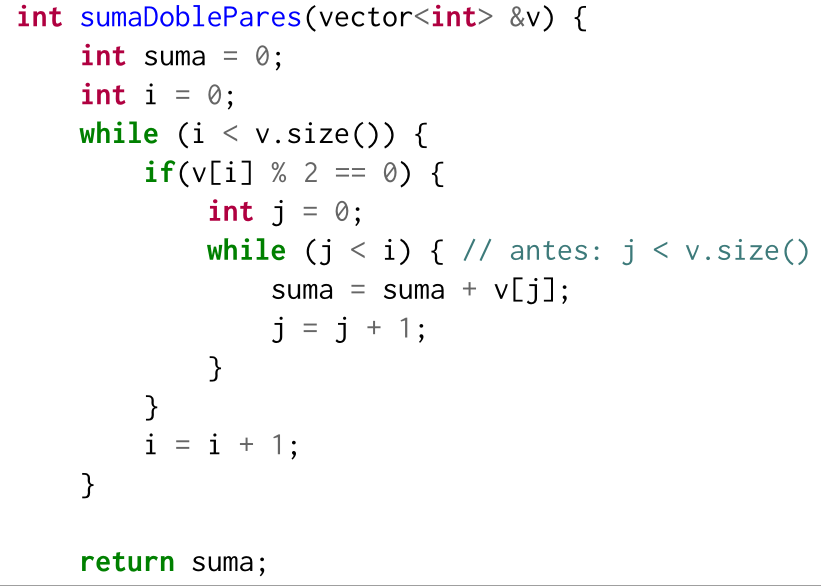
\includegraphics[width=0.7 \linewidth]{img/ej3b.png}
    \end{center}
    \begin{itemize}
        \item \textbf{Definir el tamaño de entrada $n$.} \\
            El tamaño de entrada es el tamaño del vector \texttt{|v|}. \(\implies n = |v|\)
        \item \textbf{Identificar el peor caso de ejecución del programa.} \\
            El peor caso es cuando todos los elementos del vector son pares. Esto implica que se van a sumar todos los elementos previos a un índice par.
        \item \textbf{Escribir la función de costo temporal $\mathcal{T}(n)$ asociada al peor caso.} \\
            En las primeras dos líneas se hacen dos operaciones, cuatro en total. \\
            En la guarda del \texttt{while} se hacen cuatro operaciones: se accede a \texttt{i}, \texttt{v}, se hace la operación \texttt{.size()} y se hace una comparación. Todo lo que está en este scope se ejecuta $n$ veces.\\
                En la condición del \texttt{if} se accede a dos variables, se le hace una operación y una comparación. Son, en total, cuatro operaciones. \\
                    Se define la variable \texttt{j}, cuenta como una operación. \\
                    En esta guarda del \texttt{while} se hacen tres operaciones porque se acceden a dos variables y se hace una comparación entre ellas. Todo lo que está en este scope se ejecuta $n$ veces. \\
                        Se hacen cuatro operaciones, porque se accede a \texttt{suma}, \texttt{v} y \texttt{j} y se hace una operación entre ellas. No cuenta cuando se guarda de nuevo en \texttt{suma} porque es una variable que ya se accedió. \\
                        Para incrementar \texttt{j}, se tuvo que acceder a la variable y sumarle uno. Son dos operaciones. \\
                Se incrementa \texttt{i} en un total de dos operaciones. \\
            Se devuelve \texttt{suma} en una sola operación. \\
            \\
            \(\mathcal{T}(n) = (2+2) + n(4+4+1 + n(3+4+2)+3+4+2)+1\) \\
            \(\implies \mathcal{T}(n) = 4 + n(9 + n(9)+9)+1\) \\
            \(\implies \mathcal{T}(n) = 4 + n(19 + 9n)\) \\
            \(\implies \mathcal{T}(n) = 4 + 19n + 9n^{2}\) \\
            \(\therefore \mathcal{T}(n) = 9n^{2}+19n+4\) \\
        \item \textbf{Proponer un orden de complejidad $\mathcal{O}$ para $\mathcal{T}(n)$.} \\
            \(\mathcal{T}(n) \in O(n^{2})\)
        \item \textbf{Mostrar que $\mathcal{T}(n)$ pertenece al orden de complejidad propuesto.} \\
            Quiero probar que \(0 \leq \mathcal{T}(n) \leq c \cdot O(n^{2}), (\forall n \geq n_{0})\). \\
            \(\implies 0 \leq 9n^{2}+19n+4 \leq c \cdot n^{2}, (\forall n \geq n_{0})\) \\
            \(\implies 0 \leq 9n^{2}+19n+4, (\forall n \geq n_{0})\) Vale, porque $9n^{2}+19n+4$ es una función creciente. \\
            \(\implies 9n^{2}+19n+4 \leq c \cdot n^{2}, (\forall n \geq n_{0})\) \\
            \(\implies \frac{9n^{2}+19n+4}{n^{2}} \leq c, (\forall n \geq n_{0})\) \\
            \(\implies 9+\frac{19}{n_{0}}+\frac{4}{n_{0}^{2}} \leq c, (\forall n \geq n_{0})\) \\
            Si tomo que \(n_{0} = 1 \wedge c = 32\): \\
            \(\implies 9+\frac{19}{1}+\frac{4}{1^{2}} \leq 32, (\forall n \geq n_{0})\) \\
            \(\implies 32 \leq 32, (\forall n \geq n_{0})\) Se cumple la desigualdad para todo $n \geq n_{0}$. \\
            \begin{center}
                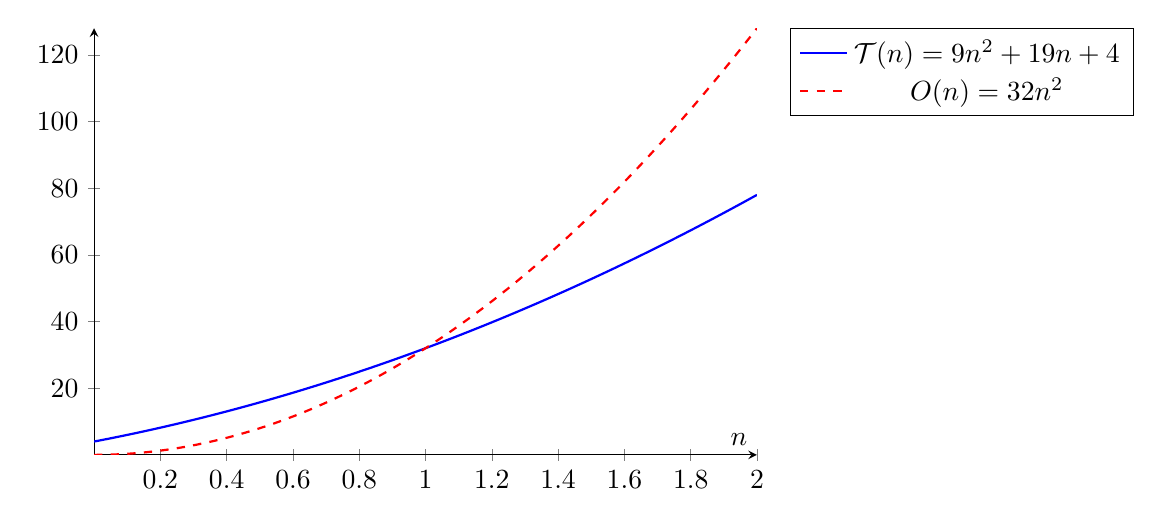
\begin{tikzpicture}
                    \begin{axis}[
                        domain=0:2,             % Rango del eje x
                        samples=100,            % Número de muestras para suavidad
                        axis lines=middle,      % Dibujar los ejes en el centro
                        xlabel={$n$},           % Etiqueta del eje x
                        ylabel={},              % Etiqueta del eje y
                        legend style={at={(1.05,1)}, anchor=north west}, % Posición de la leyenda
                        width=10cm, height=7cm, % Tamaño del gráfico
                        ]
                        % Graficar la función T(n)
                        \addplot[blue, thick] {9*x^2 + 19*x + 4};
                        \addlegendentry{$\mathcal{T}(n) = 9n^{2}+19n+4$}
                        
                        % Graficar la función O(n)
                        \addplot[red, thick, dashed] {32*x^2};
                        \addlegendentry{$O(n) = 32n^2$}
                    \end{axis}
                \end{tikzpicture}                
                \(\therefore \mathcal{T}(n) = 9n^{2}+19n+4 \in O(n^{2})\)
            \end{center} 
    \end{itemize}

\newpage

\section*{Análisis de funciones}
    \subsection*{1. \(n \in O(n \cdot log(n))\)}
        Quiero probar que \(0 \leq n \leq c \cdot O(n \cdot log(n)), (\forall n \geq n_{0})\). \\
        \(\implies 0 \leq n, (\forall n \geq n_{0})\) vale, porque $n$ es una función creciente. \\
        \(\implies n \leq c \cdot n \cdot log(n), (\forall n \geq n_{0})\) \\
        \(\implies \frac{n_{0}}{n_{0} \cdot log(n_{0})} \leq c, (\forall n \geq n_{0})\) \\
        \(\implies \frac{1}{log(n_{0})} \leq c, (\forall n \geq n_{0})\) \\
        Si tomo que \(n_{0} = 2 \wedge c = 5\) se cumple la desigualdad \(\forall n \geq n_{0}\)\\
        \begin{center}
            \begin{tikzpicture}
                \begin{axis}[
                    domain=0:10,             % Rango del eje x
                    samples=100,            % Número de muestras para suavidad
                    axis lines=middle,      % Dibujar los ejes en el centro
                    xlabel={$n$},           % Etiqueta del eje x
                    ylabel={},              % Etiqueta del eje y
                    legend style={at={(1.05,1)}, anchor=north west}, % Posición de la leyenda
                    width=10cm, height=7cm, % Tamaño del gráfico
                    ]
                    % Graficar la función T(n)
                    \addplot[blue, thick] {x};
                    \addlegendentry{$\mathcal{T}(n) = n$}
                    
                    % Graficar la función O(n)
                    \addplot[red, thick, dashed] {5*x*(ln(x)/ln(10))};
                    \addlegendentry{$O(n) = 5n \cdot log(n)$}
                \end{axis}
            \end{tikzpicture} \\              
            \(\therefore\) Esta afirmación es verdadera.
        \end{center} 
    \subsection*{2. \(n^{2}-n+2 \in O(n^{2})\)}
        Quiero probar que \(0 \leq n^{2}-n+2 \leq c \cdot O(n^{2}), (\forall n \geq n_{0})\). \\
        \(\implies 0 \leq n^{2}-n+2, (\forall n \geq n_{0})\) vale porque $n^{2}-n+2$ es una función creciente y positiva para todo $n \geq 0$. \\
        \(n^{2}-n+2 \leq c \cdot n^{2}, (\forall n \geq n_{0})\) \\
        \(\frac{n_{0}^{2}-n_{0}+2}{n_{0}^{2}} \leq c, (\forall n \geq n_{0})\) \\
        \(1-\frac{n_{0}}{n_{0}^{2}} + \frac{2}{n_{0}^{2}} \leq c, (\forall n \geq n_{0})\) \\
        \(1-\frac{1}{n_{0}} + \frac{2}{n_{0}^{2}} \leq c, (\forall n \geq n_{0})\) \\
        Si tomo que \(n_{0} = 1 \wedge c = 2\), se cumple la desigualdad para todo $n \geq n_{0}$. \\
        \begin{center}
            \begin{tikzpicture}
                \begin{axis}[
                    domain=0:2,            % Rango del eje x
                    samples=100,            % Número de muestras para suavidad
                    axis lines=middle,      % Dibujar los ejes en el centro
                    xlabel={$n$},           % Etiqueta del eje x
                    ylabel={},              % Etiqueta del eje y
                    legend style={at={(1.05,1)}, anchor=north west}, % Posición de la leyenda
                    width=10cm, height=7cm, % Tamaño del gráfico
                    ]
                    % Graficar la función T(n)
                    \addplot[blue, thick] {x^2-x+2};
                    \addlegendentry{$\mathcal{T}(n) = n^{2}-n+2$}
                    
                    % Graficar la función O(n)
                    \addplot[red, thick, dashed] {2*x^2};
                    \addlegendentry{$O(n) = 2n^{2}$}
                \end{axis}
            \end{tikzpicture} \\           
            \(\therefore\) Esta afirmación es verdadera.
        \end{center}
        
\newpage

\section*{Complejidad de algoritmos recursivos}
    \begin{center}
        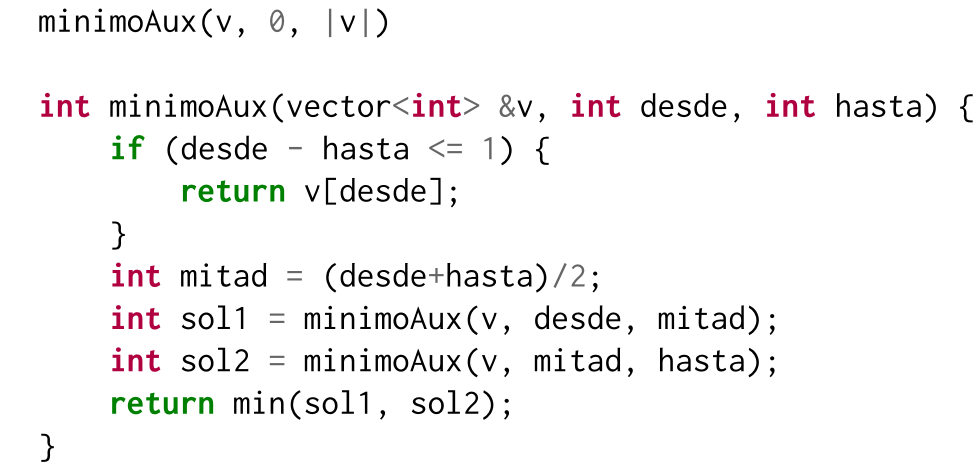
\includegraphics[width=0.7 \linewidth]{img/algoritmos-recursivos.png}
    \end{center}    
    \begin{itemize}
        \item \textbf{Definir el tamaño de entrada $n$.} \\
            El tamaño de entrada es el tamaño del vector \texttt{v}. $\implies n = |v|$
        \item \textbf{Identificar el peor caso de ejecución del programa.} \\
            El peor caso sucede cuando la variable \texttt{hasta} es igual al tamaño de \texttt{v} y cuando \texttt{desde} es igual a cero. Esto implica que se quiere buscar el mínimo de todo el vector. Peor será el caso que tenga una ejecución con un vector \texttt{v} más grande.
        \item \textbf{Escribir la ecuación de recurrencia $\mathcal{T}(n)$ asociada al peor caso.} \\
            \(
                \mathcal{T}(n) =
                \begin{cases} 
                  k & \text{si } n = 0, n = 1 \\
                  2 \mathcal{T}(n/2) + k & \text{si } n > 1
                \end{cases}
            \)
        \item \textbf{usar el árbol de recursión para dar una fórmula cerrada para $\mathcal{T}(n)$.} \\
            \(\mathcal{T}(n) = 2^{i}\mathcal{T}(n/2^{i})+k(2^{i}-1)\)
        \item \textbf{usando la fórmula cerrada, proponer un orden de complejidad $\mathcal{O}$ para $\mathcal{T}(n)$ y demostrar que pertenece.} \\
            \(\mathcal{T}(n) \in O(n)\)\\
            \(\implies 0 \leq 2kn - k \leq c \cdot n\) \\
            \(\implies 2kn - k \leq c \cdot n\) \\
            \(\implies \frac{2kn_{0} - k}{n_{0}} \leq c\) \\
            \(\implies 2k -\frac{k}{n_{0}} \leq c\) \\
            Si tomo que \(n_{0} = 1 \wedge c = k\), \\
            \(\implies 2k -\frac{k}{1} \leq k\) \\
            \(\implies k \leq k\) Se cumple \(\forall n > n_{0}\) \\
            \(\therefore \mathcal{T}(n) \in O(n)\) \\
            
    \end{itemize}

\end{document}